\documentclass{beamer}

\usepackage{framed}
\usepackage{graphicx}

\begin{document}
%====================================%
\begin{frame}[fragile]
\frametitle{Seaborn Workshop}
\large
Controlling figure aesthetics
\begin{itemize}
\item Drawing attractive figures is important. When making figures for yourself, as you explore a dataset, it’s nice to have plots that are pleasant to look at. 
\item Visualizations are also central to communicating quantitative insights to an audience, and in that setting it’s even more necessary to have figures that catch the attention and draw a viewer in.
\end{itemize}

\end{frame}
%====================================%
\begin{frame}[fragile]
\frametitle{Seaborn Workshop}
\large

Matplotlib is highly customizable, but it can be hard to know what settings to tweak to achieve an attractive plot. Seaborn comes with a number of customized themes and a high-level interface for controlling the look of matplotlib figures.
\begin{verbatim}
%matplotlib inline
import numpy as np
import matplotlib as mpl
import matplotlib.pyplot as plt
np.random.seed(sum(map(ord, "aesthetics")))
\end{verbatim}
\end{frame}
%====================================%
\begin{frame}[fragile]
\frametitle{Seaborn Workshop}
\large

Let’s define a simple function to plot some offset sine waves, which will help us see the different stylistic parameters we can tweak.
\begin{verbatim}
def sinplot(flip=1):
    x = np.linspace(0, 14, 100)
    for i in range(1, 7):
        plt.plot(x, np.sin(x + i * .5) * (7 - i) * flip)
 \end{verbatim}
This is what the plot looks like with matplotlib defaults:

sinplot()
\begin{figure}
\centering
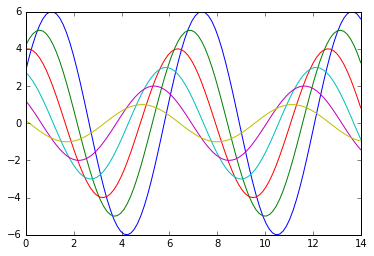
\includegraphics[width=0.7\linewidth]{images/aesthetics_8_0}
\caption{}
\label{fig:aesthetics_8_0}
\end{figure}

\end{frame}
%====================================%
\begin{frame}[fragile]
	\frametitle{Seaborn Workshop}
	\large
To switch to seaborn defaults, simply import the package.
\end{frame}
%====================================%
\begin{frame}[fragile]
	\frametitle{Seaborn Workshop}
	\large
\begin{verbatim}
import seaborn as sns
sinplot()
\end{verbatim}

\begin{figure}
\centering
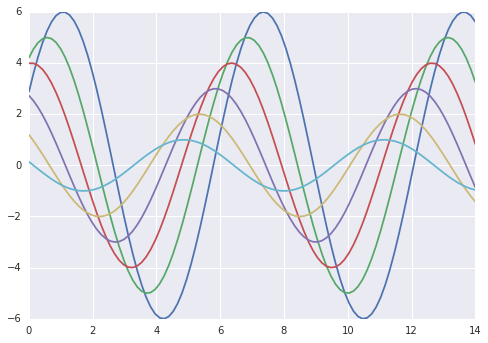
\includegraphics[width=0.7\linewidth]{images/aesthetics_10_0}
\caption{}
\label{fig:aesthetics_10_0}
\end{figure}


\end{frame}
%====================================%
\begin{frame}[fragile]
\frametitle{Seaborn Workshop}
\large
\begin{itemize}
\item The seaborn defaults break from the MATLAB inspired aesthetic of matplotlib to plot in more muted colors over a light gray background with white grid lines. 
\item We find that the grid aids in the use of figures for conveying quantitative information – in almost all cases, figures should be preferred to tables. 
\item The white-on-gray grid that is used by default avoids being obtrusive. 
\item The grid is particularly useful in giving structure to figures with multiple facets, which is central to some of the more complex tools in the library.
\end{itemize}

\end{frame}
%====================================%
\begin{frame}[fragile]
	\frametitle{Seaborn Workshop}
	\large
\begin{itemize}
\item Seaborn splits matplotlib parameters into two independent groups. 
\item The first group sets the aesthetic style of the plot, and the second scales various elements of the figure so that it can be easily incorporated into different contexts.
\end{itemize}

\end{frame}
%====================================%
\begin{frame}[fragile]
	\frametitle{Seaborn Workshop}
	\large
	\begin{itemize}
\item The interface for manipulating these parameters are two pairs of functions.
\item  To control the style, use the \texttt{axes\_style()} and \texttt{set\_style()} functions.
\item  To scale the plot, use the \texttt{plotting\_context()} and \texttt{set\_context()} functions.\
\item In both cases, the first function returns a dictionary of parameters and the second sets the matplotlib defaults.
	\end{itemize}


\end{frame}
\section{Styling figures with \texttt{axes\_style()} and \texttt{set\_style()}}
%====================================%
\begin{frame}[fragile]
	\frametitle{Seaborn Workshop}
	\large
\textbf{Styling figures with \texttt{axes\_style()} and \texttt{set\_style()}}
\begin{itemize}
\item
There are five preset seaborn themes: darkgrid, whitegrid, dark, white, and ticks. They are each suited to different applications and personal preferences. The default theme is darkgrid.
\item As mentioned above, the grid helps the plot serve as a lookup table for quantitative information, and the white-on grey helps to keep the grid from competing with lines that represent data. 
\item The whitegrid theme is similar, but it is better suited to plots with heavy data elements:
\end{itemize}
\end{frame}
%====================================%
\begin{frame}[fragile]
	\frametitle{Seaborn Workshop}
	\large
\begin{verbatim}
sns.set_style("whitegrid")
data = np.random.normal(size=(20, 6)) + np.arange(6) / 2
sns.boxplot(data=data);
\end{verbatim}
\begin{figure}
\centering
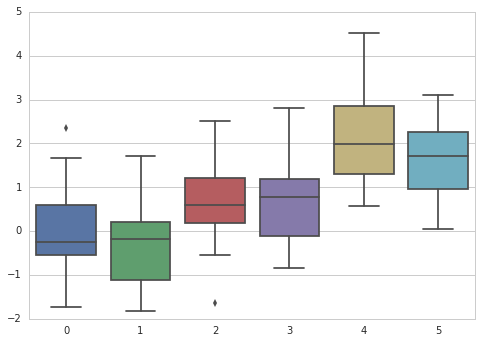
\includegraphics[width=0.7\linewidth]{images/aesthetics_12_0}
\caption{}
\label{fig:aesthetics_12_0}
\end{figure}

\end{frame}
%====================================%
\begin{frame}[fragile]
	\frametitle{Seaborn Workshop}
	\large
For many plots, (especially for settings like talks, where you primarily want to use figures to provide impressions of patterns in the data), the grid is less necessary.
\end{frame}
%====================================%
\begin{frame}[fragile]
	\frametitle{Seaborn Workshop}
	\large
\begin{verbatim}
sns.set_style("dark")
sinplot()
\end{verbatim}
\begin{figure}
\centering
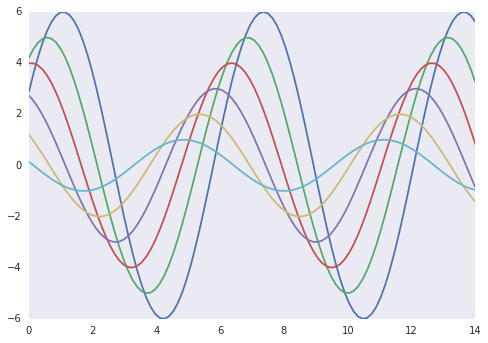
\includegraphics[width=0.7\linewidth]{images/aesthetics_15_0}
\end{figure}

\end{frame}
%====================================%
\begin{frame}[fragile]
	\frametitle{Seaborn Workshop}
	\large
\begin{verbatim}
	sns.set_style("white")
sinplot()
\end{verbatim}
\begin{figure}
\centering
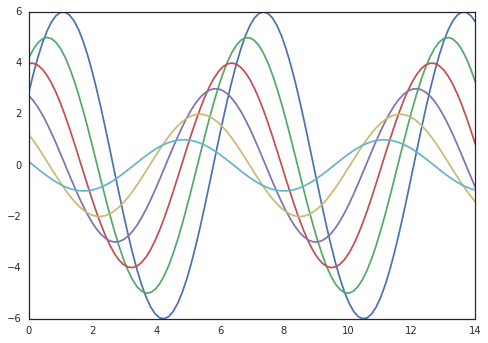
\includegraphics[width=0.7\linewidth]{images/aesthetics_17_0}
\caption{}
\label{fig:aesthetics_17_0}
\end{figure}


\end{frame}
%====================================%
\begin{frame}[fragile]
\frametitle{Seaborn Workshop}
\large
Sometimes you might want to give a little extra structure to the plots, which is where ticks come in handy:
\begin{verbatim}
sns.set_style("ticks")
sinplot()
\end{verbatim}

\begin{figure}
\centering
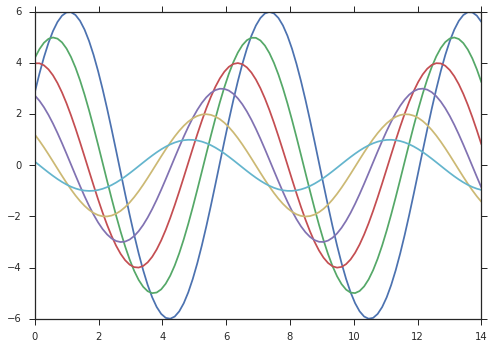
\includegraphics[width=0.7\linewidth]{images/aesthetics_19_0}
\caption{}
\label{fig:aesthetics_19_0}
\end{figure}



\end{frame}
%====================================%
\begin{frame}[fragile]
\frametitle{Seaborn Workshop}
\large
\noindent \textbf{Removing spines with despine()}\\
\begin{itemize}
\item Both the white and ticks styles can benefit from removing the top and right axes spines, which are not needed.
\item  It’s impossible to do this through the matplotlib parameters, but you can call the seaborn function \texttt{despine()} to remove them:
\end{itemize}
\end{frame}
%====================================%
\begin{frame}[fragile]
	\frametitle{Seaborn Workshop}
	\large
\begin{verbatim}
sinplot()
sns.despine()
\end{verbatim}

\begin{figure}
\centering
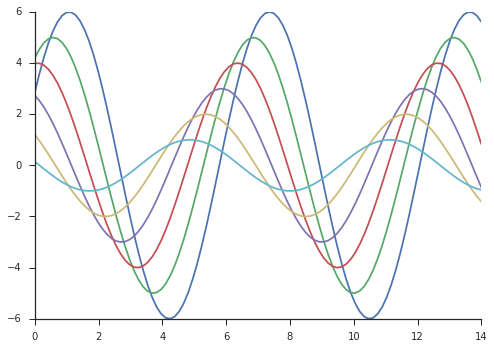
\includegraphics[width=0.7\linewidth]{images/aesthetics_21_0}
\caption{}
\label{fig:aesthetics_21_0}
\end{figure}


\end{frame}
%======================================================================= %
\end{document}